\chapter{System Analysis}
There are project details and descriptions of modules in this section.
This project will contains a mobile application which saves user location, media files and organize an event with other people, and serves side application which provides users to interact, sharing saved contents and use shared contents. 

Mobile application will saved location, notes and media files also location of media files to storage when user started trip tracking feature of application. Before starting a trip user can choose some of his/her friends to organize a trip with them. If a person added a trip this person will give a notification about accept joining to the trip. If user accepted invitation he/she can join trip as a member. Invitor is accepted as leader of team. During the trip all user's behave alone. If location sharing feature opened any member of this team can wath other members location. But as we mentioned this feature requires internet connection. At the end of trip when user want to share his/her trip data and all of sharing data shared by other members will be merged. All users can select sharing data and storing data seperately. As a result anyone could wants to store a picture but don't want to share. 

For saving location on background Android mobile application will use a saving service. User can watch his/her location path on map. If user wants to track a path which is shared from other people user can track the path by using map.

Modules created by project team as follows:
\begin{itemize}
    \item User register and login module
    \begin{itemize}
        \item User login module
        \item User register module
    \end{itemize}
    \item Trip search module
    \item Timeline preparing module
    \item Location and media save module
    \item Feature extraction module
    \item Trip management module
    \item Notification sender module
    \item Trip upload and download module
    \item Team data merging module
\end{itemize}

\newpage 
\section{Backend UML and Database Diagrams}

\begin{figure}[!htbp]
\centering
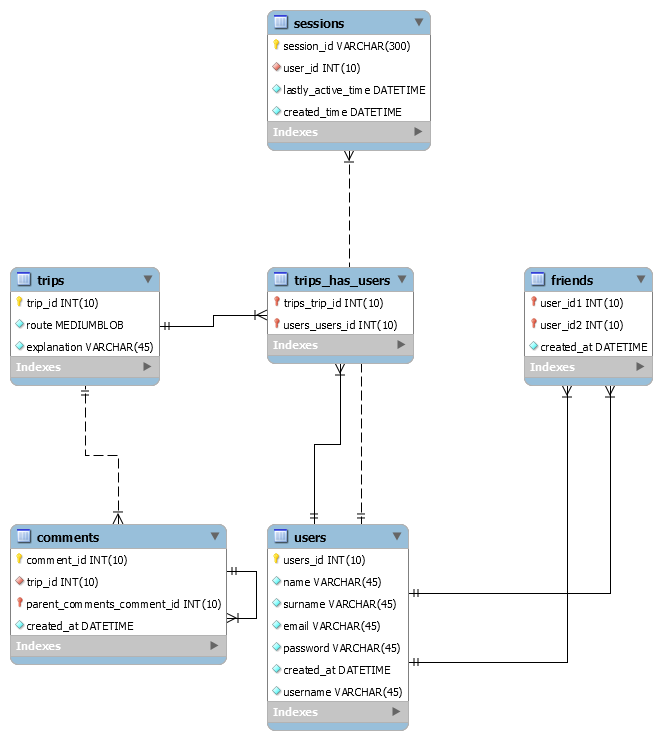
\includegraphics[width=\textwidth]{projectChapters/images/databaseDesign.png}
\caption{Database design pattern}
\end{figure}
 
 
\begin{figure}[!htbp]
\centering
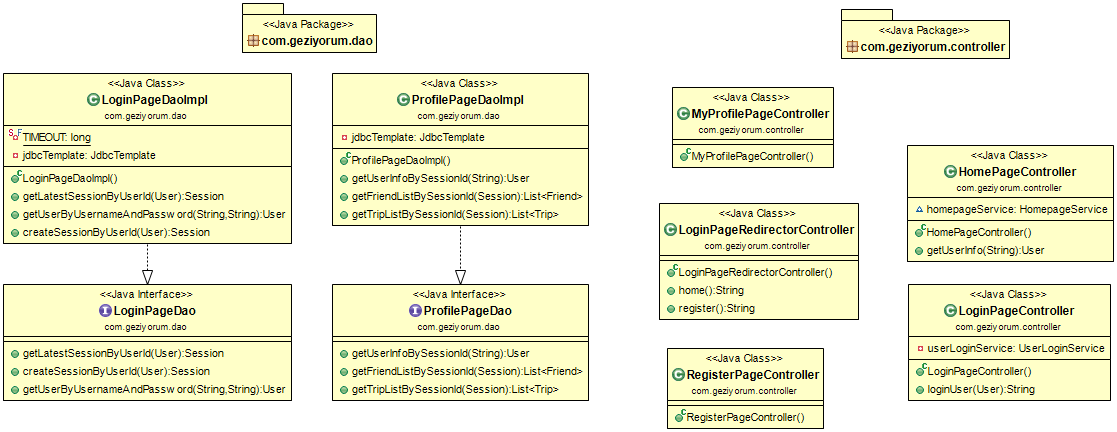
\includegraphics[width=\textwidth]{projectChapters/images/backend1.png}
\caption{Backend implementation MVC UML-1}
\end{figure}

\begin{figure}[!htbp]
\centering
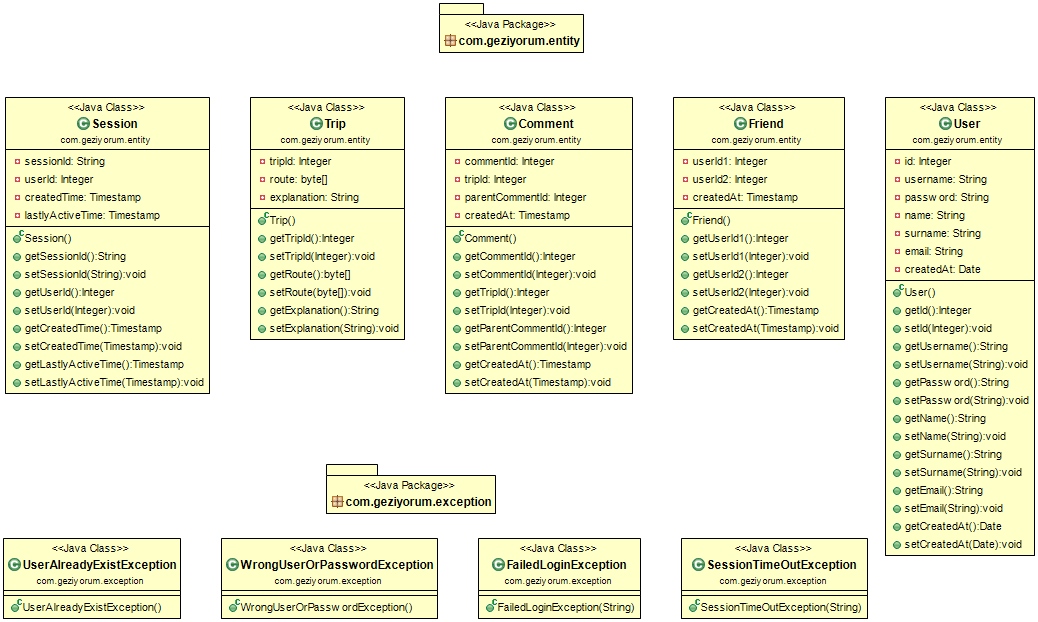
\includegraphics[width=\textwidth]{projectChapters/images/backend2.png}
\caption{Backend implementation MVC UML-2}
\end{figure}


\begin{figure}[!htbp]
\centering
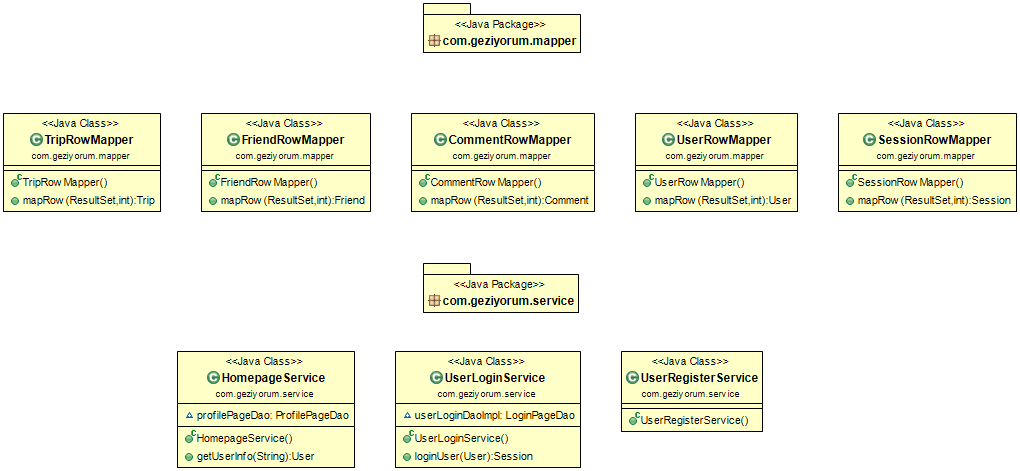
\includegraphics[width=\textwidth]{projectChapters/images/backend3.png}
\caption{Backend implementation MVC UML-3}
\end{figure} 
 
 